\documentclass[11pt,a4paper]{article}
\usepackage[utf8x]{inputenc}
\usepackage[T1]{fontenc}
%\usepackage{gentium}
\usepackage{mathptmx} % Use Times Font

\usepackage{graphicx} % Required for including pictures
\usepackage{subfigure}
\usepackage{caption}
\usepackage{hyperref} % Format links for pdf
\usepackage[british]{babel} % Multilingual bibliographies
\usepackage{natbib}
\setlength{\bibsep}{0.0pt}

\frenchspacing % No double spacing between sentences
\usepackage[margin=1in]{geometry}

\usepackage[all]{nowidow} % Tries to remove widows
\usepackage[protrusion=true,expansion=true]{microtype} % Improves typography, load after fontpackage is selected

\usepackage{lipsum} % Used for inserting dummy 'Lorem ipsum' text into the template

\title{%
 The Effect of COVID-19 on the Usage of 'Just Eat Cycles'}
 \author{s1845360 and s1900682\vspace{-6em}}
 
\date{}
%\usepackage{natbib}

\begin{document}

\maketitle

%% INSTRUCTIONS:
%%
%% 1. Please rename this file fds-project-option-1.tex,
%% fds-project-option-2.tex, or fds-project-option-3.tex, depending on
%% which project option you are doing. When you submit, please submit
%% the PDF file with the corresponding name.
%% 
%% 2. You can edit either using:
%%
%%    a. Overleaf professional, a collaborative LaTeX editor. See
%%       https://www.overleaf.com/edu/edinburgh for documentation. Create an
%%       empty document, and copy the files in this directory to it.
%%
%%    b. A LaTeX editor on your PC - you can commit changes to this
%%       repository to collaborate.
%% 
%% 3. Please keep the section and paragraph headings as they are.
%%
%% 4. The word limit for the Overview section is mandatory. For the
%% other sections word limits are suggested.
%%
%% 5. The page limits must be strictly adhered to, and depend on if
%% you are working individually, in pairs or in threes:
%%
%%   - Individual: 6 pages 
%%   - Pairs: 8 pages 
%%   - Threes: 10 pages 
%%

\section{Overview} In this report, we investigate how the usage of the bike sharing service 'Just Eat Cycles' was impacted by the COVID-19 pandemic. We hypothesised that users of 'Just Eat Cycles' would use this service to visit scenic locations and to exercise, instead of commuting. To address this hypothesis, we first examined how the activity at various stations scattered across the city changed in pre and post-lockdown periods. We expected to see that 'Just Eat Cycles' trips would not cluster as tightly around the city centre as before. Rather, we would have increased activity outside this area, specifically near scenic locations. Indeed, the number of trips at Portobello beach for example increased by \emph{11,575} in the post-lockdown period. This is contrasted to the activity at Bristo square, a popular student location in the city centre, decreasing by \emph{4735}. We also hypothesised that the proportion of \emph{long tips} in the post-lockdown period would increase. After conducting an A/B test with a bootstrap simulation, we accepted this claim with $100\%$ confidence. Similarly, there was an increase of $230.10\%$ of trips starting and ending in the same location, confirming a decreased usage for commuting purposes. This is contrasted to a $58.73\%$ increase in trips overall.
% 250 words maximum
\section{Introduction}
% Suggested 400 words
% Introduction (suggested 400 words): Background to the question to be read by someone with no
% prior knowledge of the question. It should give:
% * Context and motivation, What is the area of this data science study, and why is it interesting to investigate?
% * Brief description of any previous work in this area (e.g., in the media, scientific literature or blogs)
% * Objectives of the project – what questions are you setting out to answer?

In many metropolitan cities, there is usually a bike sharing service. In New York, there are the famous 'Citi Bikes'. London has its 'Santander Bikes' while in Edinburgh, there is the 'Just Eat Cycles'. To use this service, a user logs into to the appropriate app and finds a bike station nearest to their current location. To make use of the service, the customer rents out the use of a bike based on predefined tariffs. There are options for single trips, multiple trips and an annual pass. Customers also have the option of choosing whether they want to use a regular or an electric bike. Once the pass has been purchased, the user is able to unlock their bike and use it for the specified duration. Finally, the customer is able to return the bike to any of the stations located around the city.

\paragraph{Context and motivation}

Our study is going to investigate the effect that the COVID-19 pandemic had on the popularity of the 'Just Eat Cycles' (referred from now on as JEC). The virus posed many health concerns for individuals as not only is the virus airborne, it is also able to survive on certain surfaces, such as stainless steel, for up to 72 hours \cite{Hammett1}. With this in mind, we expected that users would avoid the use of public spaces and surfaces in order to protect themselves from the virus. However, since Edinburgh's citizens had to obey "stay-at-home" orders, we expected that the local population would want to maximise their time engaging in any physical activity outdoors during the pandemic. It is logical to infer that the popularity of the JEC would increase as this service allowed people a very accessible way to both exercise and enjoy the outdoors. The bikes also offer an isolated form of transportation compared to buses, trams and taxis. The juxtaposition of these factors provides an interesting topic of data science investigation.  

\paragraph{Previous work}Since JEC is a corporate entity that has an incentive to maximise their profits, we need to observe their actions as a business in relation to the data we are analysing. There are three examples that were very pertinent to our investigation as they affected the popularity of the service. Firstly, JEC offered free passes to all NHS workers during the pandemic in order to help them commute to and from work \cite{Stephen2}. Secondly, the company made the first 30 minutes of trips free for the general public between the 29\textsuperscript{th} of June to 13\textsuperscript{th} of July 2020. After which, the general public were provided with discounted rates for a four month period \cite{Stephen1}. Finally, the company also expanded their operations into Musselburgh as of the 21\textsuperscript{st} of September 2020 \cite{Dalton1}. Apart from this, we also viewed other data science investigations of bike sharing services for inspiration. We found an interesting academic article that examined the effect of COVID-19 on New York's 'Citi Bike'\cite{citiBike}. This is relevant to our investigation as the researchers have posed very similar questions, although in a different context. We were able to then use their ideas to complement our own findings.  

\paragraph{Objectives} In this study we are addressing the question of whether the lockdown had an effect on the nature of trips taken by users of the JEC. We will achieve this through exploring the difference between the activity at different JEC stations around Edinburgh and the difference between the number of longer trips taken between the pre- and post-lockdown periods.  

\section{Data}
% Suggested 300 words
\paragraph{Data provenance}
The data sets, based on the JEC trip data, were obtained directly from the company's web page \cite{historicalData}. The data is published under the Open Government Licence (OGL) v3.0 and it is freely available. The data sets have also been anonymised in order to protect the privacy of users. We downloaded all the data from January 2019 to March 2021 as JSON files. 

\paragraph{Data description}
Each data set, which corresponds to a calendar month between January 2019 and March 2021, contained trips with the following variables: \newline Each trip within the data has its start and end timestamp along with the duration of its use. The record also contains information about the start and end location for each trip. Each of these contain: the name of the location, a unique identification number (ID), a description of its location and the coordinates of its latitude and longitude. In 2019, there were \emph{121,110} JEC trips and in 2020, there were \emph{226,547} trips. There were \emph{137,049} pre-lockdown trips and \emph{217,535} post-lockdown trips\footnote{These data sets are with reference to the way we have split up the data, as seen in the 'Data processing' section.}.

\paragraph{Data processing} A major concern when using public data sets is whether they contain any sensitive or personal data. However, the data sets had already been anonymised. All the JSON files contain trips for an individual calendar month. Thus, we created three tables, one for 2019, one for 2020 and one for 2021 by joining all the month data sets within the respective year. After this, we created two data sets associated with either the pre-lockdown period or the post-lockdown period. The pre-lockdown dates contain trips from the 25\textsuperscript{th} of March 2019 to the 24\textsuperscript{th} of March 2020. This latter date was the first day of the national lockdown in Scotland \cite{timeline}. The post-lockdown data set includes trips from the 25\textsuperscript{th} of March 2020 to the 24\textsuperscript{th} of March 2021. We chose these specific dates to ensure that the two time periods were comparable in their time span. 
\par In addition, we checked the data set for any missing values. Our 2019 data set was clean, whilst \emph{5438} values in the 2020 data set contained null values. The null values were located in the description field for start and end locations. Since we used the actual coordinate data and did not use the description of the locations, we did not need to remove any records from our data. Finally, we ensured that all of our trip data occurred within the greater Edinburgh area (including Musselburgh) since JEC only operates out of this region. However, we observed three trips that had end locations in Liverpool. We assumed that these were erroneous trips from our data set as there are no JEC stations in Liverpool and we removed these entries from our data set.
\par During the processing, we noticed that JEC changed the names and/or exact coordinate locations of some of their stations in December 2019. We observed that our pre-pandemic data set contained two coordinate versions of the same location, of which only one was present in the post-pandemic data set. This would have proven to be problematic as we were comparing how the bike usage at individual locations changed between these two periods. To address this concern, we took each pre-pandemic location that was not present in the post-pandemic data set and found it's nearest post-pandemic location. This was done through the use of the Euclidean distance formula. We then updated all of these pre-pandemic locations to have the coordinates of their nearest neighbour. In most cases, the coordinates we updated were modified by small margins. However, adjusting the locations as described ensured more rigorous comparisons between our two data sets.  

\section{Exploration and  analysis} \label{exploration}
% Suggested 500 words for individual report; proportionately longer
% for group projects).
Initially, we focused on the number of trips taken in 2019 and 2020 respectively in Figure \ref{fds-project:fig:numberOfTrips}. This was to get a global picture of how the JEC trips were changing before investigating the effect of the pandemic. 

\begin{figure}[ht]
  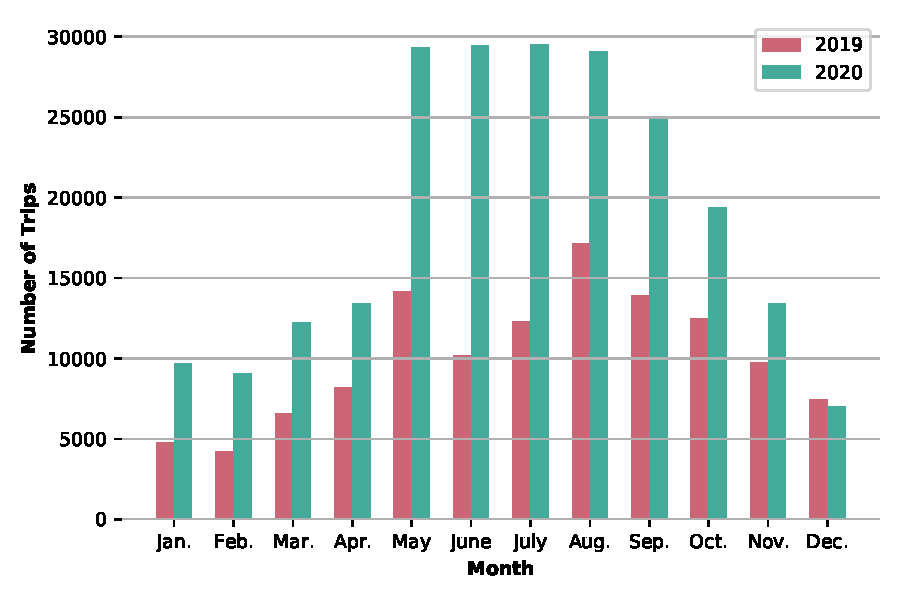
\includegraphics{number_trips.pdf}
  \caption{Bar graph comparing the number of 'Just Eat Cycle' Trips taken in 2019 and 2020.}
  \label{fds-project:fig:numberOfTrips}
\end{figure}

It is immediately visible that there are far more trips in the May to September period of 2020 when comparing it to 2019. This time period in 2020 corresponds to the first major relaxation of lockdown rules in Scotland. People were allowed to go out for exercise once a day as of the 11\textsuperscript{th} of May. On the 8\textsuperscript{th} of July, people were allowed to meet outdoors in groups of eight from a maximum of two households \cite{timeline}. The spike within this period led us to hypothesise that the main use of JEC was changing from a commuting service to one providing leisure and physical activity. Hence the main question that we wanted to address in this study is the following: how did the nature of the JEC trips change during the COVID-19 lockdown when compared to previous years.
\par Initially, we expected that the trips during the COVID-19 pandemic would become longer, and that there would be more activity at stations near scenic locations. As the lockdown progresses with its "stay-at-home" recommendations, many people would experience a sense of "lockdown fatigue". This is a natural emotion after being stuck in a very monotonous routine without opportunity to return to a sense of normality. We would expect many people to gravitate towards JEC as a means of curbing this fatigue. The bicycle scheme provides a very accessible way for individuals without their own bicycles to get outdoors and be active. We will therefore investigate (i) the changes in popularity of stations, (ii) trips starting and ending in the same location and finally (iii) the number of long trips taken by the JEC users.

\paragraph{Changes in popularity of stations} During the pre-lockdown time period, we expected that JEC were mainly used to commute between locations. This would imply that the most active stations would be clustered around the city centre, where many businesses, universities and restaurants are located. Less activity would instead be recorded near scenic locations outside of this region. We would expect the converse to be true in the post-lockdown period; the popularity of stations near scenic locations would increase as there would be much less activity near the city centre due to lockdown restrictions and closures. To answer this question, we initially plotted each station with reference to its geographical location within the map of Edinburgh. The size of each station/data point reflects how much activity \footnote{We take activity to mean any trip that has the particular station as its start or end point.} there was at that particular station during the specified time period. A visualisation of our results are seen below.

\begin{figure} [ht]
\centering
\begin{subfigure}[Pre-Lockdown]
    {
\includegraphics[width=\textwidth]{pre-lockdown_map.png}}
    \label{fds-project:fig:pre_lockdown_map}
    \end{subfigure}
\begin{subfigure}[Post-Lockdown]
    {
\includegraphics[width=\textwidth]{post-lockdown_map.png}}
    \label{fds-project:fig:post_lockdown_map}
\end{subfigure}
\begin{subfigure}[Station Activity Changes From Pre to Post-Lockdown]
    {
\includegraphics[width=\textwidth]{activity_change_map.png}}
    \label{fds-project:fig:activity_changes}
\end{subfigure}

\caption{Bubble charts showing activity for each station in Edinburgh}
\label{fig:2}
\end{figure}

\begin{table}[ht]
    \centering
    \begin{tabular}{lrrrrrrr}
\hline\hline
            \textbf{Station Name} &  \textbf{Pre-Lockdown} &  \textbf{Post-Lockdown} &  \textbf{Activity Change} \\ & \textbf{Activity} & \textbf{Activity} & \textbf{(Post - Pre)} \\
\hline
             Duke Street &                 3080.0 &                 15053.0 &                          11973.0 \\
 Portobello - Kings Road &                 8770.0 &                 20345.0 &                          11575.0 \\
       Cramond Foreshore &                 2095.0 &                 11560.0 &                           9465.0 \\
       \dots&\dots&\dots&\dots \\ 
       
    Bristo Square &                10217.0 &                  5482.0 &                          -4735.0 \\
  Waverley Bridge &                 6028.0 &                   842.0 &                          -5186.0 \\
 Logie Green Road &                 7829.0 &                  2567.0 &                          -5262.0 \\
       
\hline

\end{tabular}

    \caption{Top and bottom three station activity changes.}
\label{fds-project:table:activity_changes}
\end{table}
We can observe (Figure~\ref{fig:2}.a) that the pre-lockdown trips are clustered around the city centre. In contrast, the post-lockdown trips have a more even spread around the city (Figure~\ref{fig:2}.b). Moreover, it is immediately clear that many locations outwith the city centre, and in more scenic areas, grew substantially. The stations experiencing a decrease in activity in the post-lockdown period are all located in the city centre (Figure~\ref{fig:2}.c). Furthermore, there is an obvious increase in popularity for locations outside of the city centre. This supports our initial hypothesis as we see that stations within the city centre have become less popular, relative to the overall increase in bike usage, after the lockdown came into effect in Scotland. JEC users have chosen to spend more time in scenic locations. Table \ref{fds-project:table:activity_changes} complements the visual results shown in Figure \ref{fig:2}. The three stations that saw the largest increase in activity were all locations within popular outdoor locations. The 'Duke Street' station is adjacent to the Leith Links park. Portobello and Cramond Foreshore are both near popular beaches in Edinburgh. In contrast, the three locations with negative changes in the post-lockdown period are all within the city centre. Bristo Square is at the heart of the University of Edinburgh's central campus. Waverly bridge is right beside Edinburgh's central railway station and Logie Green Road is a station within a residential area in close proximity to a student accommodation (Beaverbank). The usage of these stations decreased substantially in the post-lockdown period when compared to their pre-lockdown usage, even though the overall number of trips taken in the post-lockdown period by JEC users increased significantly, as seen in Figure~\ref{fds-project:fig:numberOfTrips}. These results support our main hypothesis as they showed that the JEC users chose to use the bike hire service as a leisurely activity and a means of exercise rather than for commuting. Please note the trips near Queensferry in the top left-hand corner of Figure \ref{fig:2}.b. These stations did not exist prior to September 2020 \cite{Dalton1}, thus it would be erroneous to include them in our discussion as they do not have a reference point in the pre-lockdown data set. 

\paragraph{Trips starting and ending in the same location} Next, we compared the number of trips that started and ended in the same location across the two time periods. Commuters travel between two distinct locations $a$ and $b$. Trips that start and end in the same location $c$ are generally not for this same purpose. It is more likely that they are used for leisure or exercise. Within the pre-lockdown period, there were \emph{12,450} trips that started and ended in the same location. In the post-lockdown period, this number increased to \emph{41,097}. However, this increase from 2020 could also be due to the company's natural rising popularity, irrespective of the nature of trips changing \footnote{See \emph{\nameref{evaluation}}}. To control for this possibility, we compared the percentage increase from the pre-lockdown period to the post-lockdown period for the total number of trips to the percentage increase of trips that started and ended in the same location. The percentage increase for total number of trips was $58.73\%$. The percentage increase for the number of trips that started and ended in the same location was $230.10\%$. This indicates that there was in fact an increased number of non-commuting trips due to the pandemic. If this was not the case we would expect the two percentage increases to be closer in value, controlling for other factors. 

\paragraph{Duration of Trips} To test whether the trips were longer during the post-lockdown period, we decided to conduct an A/B test. In our test, we considered longer trips to be those greater than 30 minutes. We assumed that a trip taken for commuting purposes would take less than 30 minutes while  trips longer than 30 minutes are for non-commuting purposes \footnote{Such examples include exercise, leisure etc.}. In our A/B test, $A$ represented the post-lockdown period and $B$ was the pre-lockdown period. We assume each trip to be independent and observed the Bernoulli random variable of a trip either being a \emph{long trip} (greater than 30 minutes) or not a \emph{long trip}. To obtain the probability of a trip being long for each period, we found the number of long trips in each data set which was then divided by the total number of trips. As the number of trips in each period was large, we can take these probabilities to be the limiting relative frequencies (Figure 4). The probability of there being a \emph{long trip} in post-lockdown, $P_A$, is $0.44$. The probability of there being a \emph{long trip} in pre-lockdown, $P_B$, is $0.24$ \footnote{Decimals were rounded to two decimal places for legibility.}. We used the \emph{bootstrap} method, sampling a number of \emph{long trips} from a binomial distribution for each time period with their respective probabilities and $n$ equal to the average number of trips per month, $13,643$. We then calculated the difference between the sampled number of \emph{long trips}, normalised by $n$, which represented a single data point. We repeated this process $1000$ times and plotted the resulting bootstrap distribution (Figure \ref{fds-project:fig:bootstrap}). 

\begin{figure}[ht]
  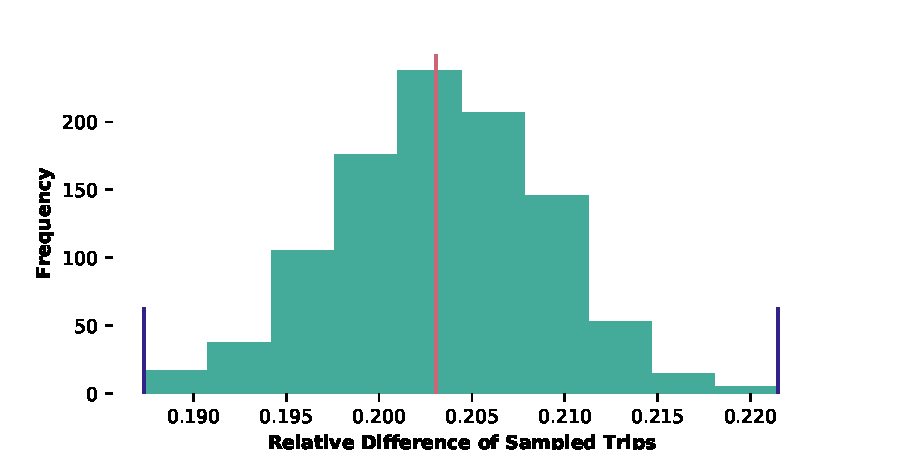
\includegraphics{bootstrap.pdf}
  \caption{A/B test bootstrap simulation comparing the difference in number of \emph{long trips} in the post-lockdown and pre-lockdown periods. Samples were drawn from two binomial distributions with $P_A$ (post-lockdown) $= 0.44$, $P_B$ (pre-lockdown) $= 0.24$, and $n$ (average trips per month) $=13,643$. }
  \label{fds-project:fig:bootstrap}
\end{figure}


In Figure~\ref{fds-project:fig:bootstrap}, the pink line represents the difference between $P_A$ and $P_B$. The purple lines represent the \emph{minimum} and \emph{maximum} values obtained. We can see that $0$, representing that there is no difference between the aforementioned proportions, is not included within our interval at all. Thus, we can say with $100\%$ confidence that the trips during a month-long period in post-lockdown contain more \emph{long trips} when compared to pre-lockdown. This supports our initial investigative question as it shows that consumers were spending a far greater duration of time on the JEC. This, coupled with the station activity changes discussed above, shows that individuals were using the bike hire service as a means to visit more scenic locations. To complement our A/B test, we also calculated the limiting relative frequency of the number of \emph{long trips} in pre-lockdown and post-lockdown. The visualisation of this is seen in Figure  \ref{fds-project:fig:relativeFrequency} where will  will allow n to be the number of trips. As $\lim_{n \to +\infty}$, we see that the proportion of \emph{long trips} in post-lockdown and pre-lockdown tend to two distinct asymptotes. These asymptotes correspond to the values of $P_A$ and $P_B$ respectively used in our AB test. 
\begin{figure}[ht]
  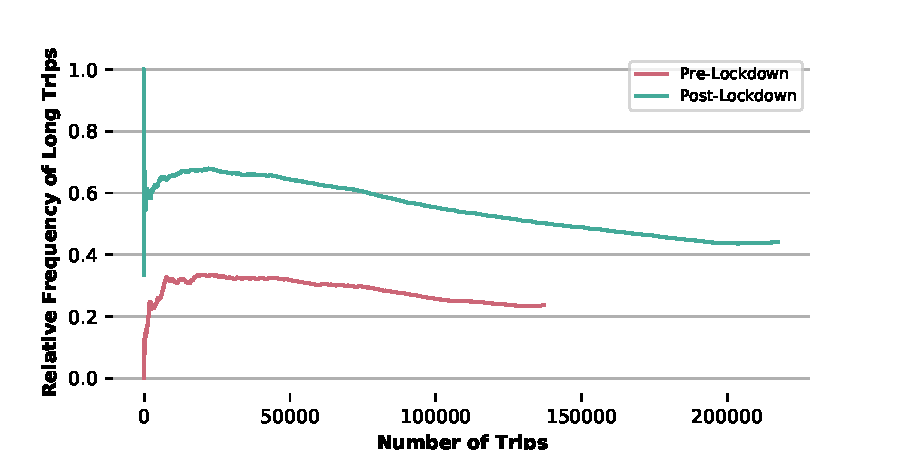
\includegraphics{relative_frequencies.pdf}
  \caption{A visual of the relative frequencies for long trips in the pre-lockdown and post-lockdown periods.}
  \label{fds-project:fig:relativeFrequency}
\end{figure}

\section{Discussion and conclusions}
% Suggested 400 words.

\paragraph{Summary of findings}
The effect of the COVID-19 pandemic had a profound impact on JEC as it changed the bike sharing service's primary use. Preceding lockdown, the service was primarily used to assist commuters, as it does in many other metropolitan cities. The bicycles provide a very accessible and cost-effective means to get from point $A$ to point $B$ and are used by both business people and students alike, visible by the clustering of trips around Edinburgh's city centre. However, our investigation showed that the usage of the JEC shifted in the post-lockdown period to focus on leisure and exercise. This was apparent for two key reasons. Firstly, the clustering of trips was no longer as tight around the city centre. This was seen in Figure \ref{fig:2} by the comparison between the pre-lockdown station activity to the post-lockdown station activity. Moreover, we also observed that users of the service increased their tendency to travel to more scenic locations. This was observed by increased activity at popular scenic locations in Edinburgh such as Portobello beach and various parks located around the city. This notion is also supported by our second question showing that the likelihood of a long trip increased in post-lockdown. Users took many more \emph{long trips} in the post-lockdown period. This, coupled with the increased number of trips  starting and ending in the same location, indicated that the trips taken were no longer for commuting but for leisure and to break the 'lockdown fatigue'.



\paragraph{Evaluation of own work: strengths and limitations}\label{evaluation}
One of our strengths is that we took care to mitigate the influence of confounding variables on our findings. Before conducting our study, we explored the data to see whether there was a general trend of increase in popularity. We observed that the popularity of the JEC was naturally increasing over time. Thus, when comparing the number of trips that started and ended in the same locations, we took measures to address this factor by comparing this to the percentage increase of trips between the pre-lockdown and post-lockdown periods. An additional strength of our investigation was the extensive prepossessing we conducted before proceeding with our experiments. We observed that there were a number of locations that changed between pre-lockdown and post-lockdown due to the JEC expanding their operations. We also observed that some locations ceased to exist. In order to ensure a proper comparison, we grouped the data for locations in the pre-lockdown data set with their nearest locations in the post-lockdown data set. This would allow us to account for all trip data for stations within the JEC bike hire service.\par Our investigation has two main limitations. The first is that the popularity of the JEC was already increasing prior to the COVID-19 lockdown (Figure~\ref{fds-project:fig:numberOfTrips}). The number of trips in January and February of 2020 were almost double the number of trips within the respective months in 2019. However, we believe that the COVID-19 pandemic actually amplified the company's success. As we have already shown above, the JEC provided Edinburgh's citizens without their own bikes a very accessible way to both exercise and visit scenic locations. The JEC needed to expand their operations to cope with this demand, as seen by their expansion into Musselburgh \cite{Dalton1}. A similar limitation would be viewed when we compared the percentage increase of trips that started and ended in the same location in the pre-lockdown and post-lockdown period. However, as we stated above, we made sure to compare this to the percentage increase of total number of trips. This comparison allowed us to show that the nature of trips were in fact changing, and that the percentage increase in the trips starting and ending in the same location was not just due to the increased popularity of the JEC.

\paragraph{Comparison with any other related work} A similar trend was viewed with New York's 'Citi Bikes' \cite{citiBike}. In the aforementioned study, João Filipe Teixeira and Miguel Lopes observed that that there was a $34\%$ increase in the duration of trips in March 2020 compared to the duration of trips in March 2019. These dates correspond to our time periods of March 2020 being in post-lockdown and March 2019 being in pre-lockdown. Although we investigated the difference in number of \emph{long trips} taken, our findings match with the findings of the New York 'Citi Bikes' as in both New York and Edinburgh, there were more trips with a longer duration as a result of the pandemic.

\paragraph{Improvements and extensions} To extend our findings, we identified three interesting paths of exploration one could take. Firstly, our findings have shown that there is a definite shift in the nature of JEC when comparing pre-lockdown to post-lockdown. It would be interesting to observe how this trend differed on weekdays compared to weekends rather than grouping the entire period as one.\par Secondly, we could investigate how commuting methods in Edinburgh changed as a result of the pandemic. We only observed changes in bike hire services, but it would be interesting to contrast these findings with the changes seen in bus, tram and taxi usage in Edinburgh. \par Throughout the lockdown in Scotland, there have been various restrictions introduced that prevent certain activities in response to the rising COVID-19 cases. Such restrictions include the closure of bars and restaurants for example. In our investigation, we only considered the announcement of lockdown on the 24\textsuperscript{th} of March 2020 and the allowance of outdoor exercise on the 11\textsuperscript{th} of May 2020. It would be interesting to observe how the number of JEC trips was affected by the announcements of additional lockdown restrictions. An example of such a restriction would be the curfew imposed on pubs and restaurants on the 22\textsuperscript{nd} of September 2020 \cite{timeline}. Similarly, it would be interesting to observe how the number of JEC trips fluctuated in response to the number of COVID-19 cases at a particular time. The two trends could be plotted against one another and their difference observed. 

\bibliographystyle{unsrt}
\bibliography{fds-project}
\end{document}
